\documentclass[11pt,a4paper]{article}

% --- Paquetes Esenciales ---
\usepackage[spanish,es-tabla]{babel}
\usepackage[utf8]{inputenc}
\usepackage[T1]{fontenc}
\usepackage{geometry}
\geometry{top=2.5cm, bottom=2.5cm, left=2.5cm, right=2.5cm}

\usepackage{amsmath,amssymb,amsfonts,amsthm}
\usepackage{graphicx}
\usepackage{booktabs}
\usepackage{tabularx}
\usepackage{multirow}
\usepackage{xcolor}
\usepackage{hyperref}
\usepackage{caption}
\usepackage{subcaption}
\usepackage{listings}
\usepackage{microtype}
\usepackage{cite}

% --- Definición de Colores ---
\definecolor{primary}{RGB}{20, 50, 90}
\definecolor{secondary}{RGB}{120, 30, 30}
\definecolor{codebg}{RGB}{245, 247, 250}
\definecolor{codeframe}{RGB}{210, 215, 225}

% --- Configuración de Enlaces ---
\hypersetup{
    colorlinks=true,
    linkcolor=primary,
    citecolor=secondary,
    urlcolor=primary
}

% --- Entornos Teóricos ---
\newtheorem{theorem}{Teorema}
\newtheorem{definition}{Definición}
\newtheorem{property}{Propiedad}

% --- Configuración de Listings (Código) ---
\lstset{
    backgroundcolor=\color{codebg},
    frame=single,
    rulecolor=\color{codeframe},
    basicstyle=\ttfamily\footnotesize,
    keywordstyle=\color{primary}\bfseries,
    commentstyle=\color{gray}\itshape,
    stringstyle=\color{secondary},
    breaklines=true,
    numbers=left,
    numberstyle=\tiny\color{gray},
    numbersep=5pt,
    tabsize=2,
    showstringspaces=false
}

% ==============================================================================
% DATOS DEL INFORME
% ==============================================================================
\title{
    \vspace{-1.5cm}
    \textbf{\Large Evaluación 2: Resolución del Problema del Árbol de Steiner en Grafos}\\
    \large Instancia de Optimización E18 (SteinLib)
}

\author{
    \textbf{Martin Verdugo} \quad \textbf{Nicolas Montecino} \quad \textit{[Integrante 3 - Opcional]} \\[0.2cm]
    \textit{Carrera de Ingeniería Civil Informática} \\
    \textit{Asignatura: Inteligencia Artificial} \\
    \textit{Docente: Dr(c). Francisco Philip Vásquez Iglesias}
}

\date{Viernes 16 de Octubre de 2026}

\begin{document}

\maketitle

\begin{abstract}
El presente trabajo aborda la resolución computacional del \textbf{Problema del Árbol de Steiner en Grafos (STPG)}, un problema fundamental de optimización combinatoria de clase \textbf{NP-Hard}. Se analiza la instancia real \texttt{e18.stp} del repositorio de referencia internacional \textit{SteinLib}, compuesta por $2.500$ nodos, $62.500$ aristas y $417$ nodos terminales obligatorios. Se implementa una solución base fundamentada en el Árbol Generador Mínimo (MST) mediante el algoritmo de Kruskal optimizado con la estructura Disjoint Set Union (DSU) con unión por rango, alcanzando un costo inicial de $2.515$ en $\sim 4$ ms. Posteriormente, se demuestra y aplica un algoritmo lineal de poda iterativa de hojas Steiner no terminales que reduce el costo en un $-60,04\%$ ($1.005$ unidades de costo) en $0,2$ ms, preservando la conexidad y aciclicidad estricta. Finalmente, se modelan y evalúan heurísticas de mejora para aproximarse al óptimo teórico global de $564$.
\end{abstract}

\vspace{0.3cm}
\noindent\textbf{Palabras clave:} Árbol de Steiner, Grafos Ponderados, Algoritmo de Kruskal, Poda Estructural, Heurística KMB, Inteligencia Artificial.

\vspace{0.5cm}

% ==============================================================================
% SECCIÓN 1: DESCRIPCIÓN DEL PROBLEMA Y MODELACIÓN
% ==============================================================================
\section{Descripción del Problema y Modelación Matemática}
\label{sec:modelacion}

\subsection{Definición del Problema}
En el diseño y planificación de redes de infraestructura física (fibra óptica, tendido eléctrico y transporte de fluidos), el objetivo cardinal radica en interconectar un conjunto de nodos de interés prioritario minimizando el costo total del cableado. Formalmente, este desafío se modela como el \textbf{Problema del Árbol de Steiner en Grafos} (\textit{Steiner Tree Problem in Graphs}, STPG).

A diferencia del clásico problema del Árbol Generador Mínimo (MST), donde todos los vértices del grafo deben ser incluidos obligatoriamente en la red final, en el STPG los vértices se clasifican en dos conjuntos disjuntos:
\begin{enumerate}
    \item \textbf{Nodos Terminales ($T$):} Puntos obligatorios que deben quedar mutuamente comunicados.
    \item \textbf{Nodos de Steiner ($S$):} Puntos auxiliares u opcionales cuya inclusión sólo se justifica si actúan como puentes topológicos que disminuyan el costo total de la red.
\end{enumerate}

\subsection{Formulación Matemática}
Sea $G = (V, E, w)$ un grafo no dirigido y ponderado, donde $V$ es el conjunto finito de vértices ($|V| = n$), $E \subseteq V \times V$ es el conjunto de aristas ($|E| = m$), y $w: E \to \mathbb{Z}^+$ es una función de costo que asigna un peso estrictamente positivo a cada conexión.

Dado un subconjunto de terminales $T \subseteq V$ con $|T| \ge 2$, el problema consiste en hallar un subgrafo conexo y acíclico $T_{\text{opt}} = (V_A, E_A)$ tal que:
\begin{equation}
    \min_{E_A \subseteq E} \sum_{e \in E_A} w(e)
\end{equation}
sujeto a las restricciones:
\begin{align}
    T &\subseteq V_A \subseteq V \\
    (V_A, E_A) &\quad \text{es un grafo conexo} \\
    |E_A| &= |V_A| - 1 \quad (\text{estructura de árbol acíclico})
\end{align}

\subsection{Complejidad Computacional y Espacio de Búsqueda}
El STPG fue demostrado como \textbf{NP-Hard} por Richard M. Karp en 1972 \cite{karp1972reducibility}. El espacio de búsqueda combinatorio consiste en encontrar el subconjunto óptimo de nodos Steiner $S^* \subseteq S$ tal que el MST inducido sobre $T \cup S^*$ minimice la suma de pesos:
\begin{equation}
    |\Omega| = 2^{|V \setminus T|} = 2^{|S|}
\end{equation}
Para la instancia bajo estudio (\texttt{e18.stp}), con $|S| = 2.083$, el espacio de combinaciones posibles es de orden $2^{2.083} \approx 10^{627}$, lo que imposibilita de manera absoluta cualquier intento de búsqueda exhaustiva o fuerza bruta. En consecuencia, se exige el diseño de heurísticas constructivas, podas estructurales y algoritmos de aproximación.

% ==============================================================================
% SECCIÓN 2: REPRESENTACIÓN DEL GRAFO
% ==============================================================================
\section{Representación del Grafo y Estructuras de Datos}
\label{sec:grafo}

\subsection{Características de la Instancia E18 (SteinLib)}
Se utilizó la instancia de referencia \textbf{E18} perteneciente a la Serie E del repositorio \textit{SteinLib} \cite{steinlib}, creada por J. E. Beasley \cite{beasley1990orlibrary}. Los parámetros constitutivos son:
\begin{itemize}
    \item \textbf{Total de vértices ($|V|$):} $2.500$ nodos.
    \item \textbf{Terminales obligatorios ($|T|$):} $417$ nodos.
    \item \textbf{Nodos Steiner opcionales ($|S|$):} $2.083$ nodos ($83,32\%$ del grafo).
    \item \textbf{Total de aristas ($|E|$):} $62.500$ aristas con pesos enteros $w \in [1, 10]$.
    \item \textbf{Peso acumulado del grafo completo:} $344.231$ unidades.
\end{itemize}

\subsection{Diseño en Memoria y Complejidad Espacial}
Para maximizar la eficiencia temporal en el procesamiento de $62.500$ conexiones, se implementó en C++17 una representación dual en memoria indexada estrictamente en base 1:
\begin{enumerate}
    \item \textbf{Lista secuencial de aristas (\texttt{edge\_list}):} Vector continuo de tipo \texttt{std::vector<Edge>}, optimizado para el ordenamiento previo del algoritmo de Kruskal en memoria contigua de alta localidad de caché.
    \item \textbf{Lista de adyacencia ponderada (\texttt{adj}):} Estructura \texttt{std::vector<std::vector<Neighbor>>} de tamaño $|V| + 1$ para búsquedas en anchura (BFS) y cálculo de caminos mínimos vía Dijkstra.
    \item \textbf{Vector de pertenencia booleano (\texttt{is\_terminal}):} Vector \texttt{std::vector<bool>} que permite discriminar en tiempo constante $O(1)$ si un vértice $u$ es un terminal obligatorio o un nodo Steiner auxiliar.
\end{enumerate}

\subsection{Ordenamiento Determinista}
Para evitar comportamientos indefinidos o variaciones de desempate entre diferentes compiladores y plataformas (GCC Linux vs. MinGW Windows), se sobrecargó el operador de orden de las aristas garantizando ordenamiento estricto por peso y por identificador de vértices:
\begin{equation}
    e_1 < e_2 \iff (w_1 < w_2) \lor (w_1 = w_2 \land u_1 < u_2) \lor (w_1 = w_2 \land u_1 = u_2 \land v_1 < v_2)
\end{equation}

% ==============================================================================
% SECCIÓN 3: ALGORITMO BASE (MST)
% ==============================================================================
\section{Algoritmo Base Implementado (Árbol Generador Mínimo)}
\label{sec:mst}

\subsection{Fundamento Metodológico y Formulación Dual: Kruskal vs. Prim}
De acuerdo a lo estipulado textualmente en la pauta de la asignatura (\textit{Clase 3 Búsqueda no informada}, diapositiva 310: \textit{"Árbol de expansión mínima (MST) utilizando Kruskal o Prim"}), se implementaron ambas formulaciones clásicas sobre el grafo global $G$ para comparar su impacto estructural:

\begin{enumerate}
    \item \textbf{Algoritmo de Kruskal \cite{kruskal1956shortest}:} Opera con enfoque global ordenando las $|E| = 62.500$ aristas y uniendo componentes conexas disjuntas mediante una estructura \textbf{Disjoint Set Union (DSU)} optimizada con \textit{Path Compression} y \textit{Union by Rank} en tiempo $O(|E| \log |E| + |E|\alpha(|V|))$.
    \item \textbf{Algoritmo de Prim \cite{prim1957shortest}:} Crece radialmente a partir de un vértice semilla terminal ($r \in T$, por defecto el nodo $1476$), manteniendo en todo momento una única componente conexa en expansión. Emplea una cola de prioridad (\textit{min-heap}) sobre las aristas del corte en tiempo $O(|E| \log |V|)$. Además, se incorporó una variante con desempate orientado a terminales, que prioriza conectar hacia nodos de $T$ en caso de igualdad de pesos.
\end{enumerate}

\subsection{Propiedad de Factibilidad y Equivalencia de Costo Global}
Dado que el grafo original $G$ es conexo, el MST generado por cualquiera de los dos métodos conecta la totalidad de los $2.500$ nodos con exactamente $|V| - 1 = 2.499$ aristas. Como abarca a todos los vértices, forzosamente contiene los $417$ nodos terminales, constituyendo una solución factible inmediata.

Teóricamente, tanto Kruskal como Prim garantizan encontrar un Árbol Generador Mínimo global óptimo. En la instancia \texttt{e18.stp}, ambas implementaciones alcanzan de forma exacta el mismo costo global de $\mathbf{2.515}$, lo que verifica la consistencia matemática y satisface el requisito base de 4 puntos de la pauta docente (Tabla \ref{tab:mst_base}). Sin embargo, la topología interna generada difiere sustancialmente, como se analiza en la siguiente sección.

\begin{table}[h]
\centering
\small
\caption{Métricas obtenidas para la solución base MST en la instancia E18 mediante Kruskal y Prim.}
\label{tab:mst_base}
\begin{tabular}{lcccc}
\toprule
\textbf{Solución} & \textbf{Costo Total} & \textbf{Aristas} & \textbf{Nodos Conectados} & \textbf{Tiempo de Cómputo} \\
\midrule
MST Base (Kruskal) & $2.515$ & $2.499$ & $2.500$ (100\% del grafo) & $4,80$ ms \\
MST Base (Prim Estándar) & $2.515$ & $2.499$ & $2.500$ (100\% del grafo) & $4,09$ ms \\
MST Base (Prim Desempate Terminal) & $2.515$ & $2.499$ & $2.500$ (100\% del grafo) & $4,78$ ms \\
\bottomrule
\end{tabular}
\end{table}

% ==============================================================================
% SECCIÓN 4: ESTRATEGIA DE SOLUCIÓN FACTIBLE Y PODA
% ==============================================================================
\section{Estrategia de Solución Factible y Poda Estructural}
\label{sec:poda}

\subsection{Teorema de Optimalidad de Hojas Steiner}
Si bien el MST base es factible, incorpora innecesariamente los $2.083$ nodos Steiner, muchos de los cuales terminan en las ramas periféricas del árbol sin cumplir ningún rol conector entre los terminales.

\begin{theorem}[Propiedad de Optimalidad de Hojas Steiner]
En cualquier subgrafo conexo solución $T' = (V', E')$ del problema del árbol de Steiner, ninguna hoja (nodo con $\text{grado}(u) = 1$) puede ser un nodo de Steiner ($u \notin T$).
\end{theorem}

\begin{proof}
Supóngase por contradicción que existe una solución conexa factible $T'$ tal que existe una hoja $u \in V'$ con $\text{grado}_{T'}(u) = 1$ y $u \notin T$. Sea $e = (u, v) \in E'$ la única arista incidente a $u$. Al eliminar la arista $e$, el subgrafo resultante $T'' = (V' \setminus \{u\}, E' \setminus \{e\})$ mantiene a todos los nodos de $V' \setminus \{u\}$ en su misma componente conexa original. Como $u \notin T$, el conjunto de terminales no se ve alterado ($T \subseteq V' \setminus \{u\}$). Dado que los costos de las aristas son estrictamente positivos ($w(e) > 0$), el costo acumulado de $T''$ satisface:
\begin{equation}
    w(T'') = w(T') - w(e) < w(T')
\end{equation}
Por ende, $T'$ contiene costo superfluo y la eliminación recursiva de $u$ preserva la factibilidad estricta.
\end{proof}

\subsection{Algoritmo de Poda Iterativa en Tiempo Lineal}
Para eliminar todas las hojas no terminales en tiempo $O(|V| + |E|)$, se diseñó un algoritmo con cola de grados:
\begin{enumerate}
    \item Se calcula el grado de cada vértice en el árbol solución.
    \item Se inicializa una cola (\texttt{std::queue}) con todos los vértices tales que $\text{grado}(u) = 1$ y \texttt{is\_terminal[u] == false}.
    \item Se extrae cada nodo de la cola, se remueve su arista incidente, se decrementa el grado de su vecino adyacente $v$, y si $v$ pasa a tener grado 1 sin ser terminal, se encola para su posterior remoción.
\end{enumerate}

\subsection{Resultados Experimentales de la Poda y Superación del Hito 892}
Al ejecutar la poda de hojas sobre las distintas variantes de MST para la instancia \texttt{e18.stp}, se obtienen los resultados expuestos en la Tabla \ref{tab:poda_results}.

\begin{table}[h]
\centering
\small
\caption{Impacto de la poda estructural de hojas Steiner sobre las soluciones base de Kruskal y Prim.}
\label{tab:poda_results}
\begin{tabular}{lccccc}
\toprule
\textbf{Método} & \textbf{Costo} & \textbf{Reducción \%} & \textbf{Aristas} & \textbf{Nodos ($T$ / $S$)} & \textbf{Tiempo} \\
\midrule
Kruskal Base & $2.515$ & $0,00\%$ & $2.499$ & $417$ / $2.083$ & $4,80$ ms \\
Kruskal Podado (Hojas) & $1.005$ & $-60,04\%$ & $1.003$ & $417$ / $587$ & $0,35$ ms \\
\midrule
Prim Base & $2.515$ & $0,00\%$ & $2.499$ & $417$ / $2.083$ & $4,78$ ms \\
Prim Podado (Estándar) & $922$ & $-63,34\%$ & $920$ & $417$ / $504$ & $0,14$ ms \\
\textbf{Prim Podado (Desempate Terminal)} & $\mathbf{779}$ & $\mathbf{-69,03\%}$ & $\mathbf{777}$ & $\mathbf{417\text{ / }361}$ & $\mathbf{0,14\text{ ms}}$ \\
\midrule
\textit{Hito Pauta Oficial (Poda Estructural)} & \textit{892} & \textit{-64,53\%} & \textit{-} & \textit{-} & \textit{5 puntos} \\
\bottomrule
\end{tabular}
\end{table}

\noindent\textbf{Análisis Topológico y Superación de la Cota 892:}  
La comparativa entre Kruskal y Prim revela hallazgos teóricos y prácticos de gran relevancia:
\begin{enumerate}
    \item \textbf{Dispersión Global de Kruskal ($1.005$):} Kruskal selecciona aristas globalmente baratas sin importar la distancia a los terminales. Esto genera múltiples componentes disjuntas que luego se enlazan mediante largas cadenas de nodos Steiner en la periferia, reteniendo $587$ nodos Steiner incluso tras podar todas las hojas de grado 1.
    \item \textbf{Crecimiento Radial de Prim ($922$):} Al germinar desde un terminal semilla ($1476$), Prim expande la frontera de corte de forma conexa y radial. Esta propiedad natural reduce de inmediato la dispersión y conduce a un árbol podado de $922$ unidades de costo ($920$ aristas).
    \item \textbf{Desempate Orientado a Terminales ($\mathbf{779}$ vs. Hito $892$):} En el grafo \texttt{e18}, existen múltiples aristas con pesos idénticos. Al romper empates favoreciendo explícitamente aristas incidentes a terminales obligatorios (\texttt{is\_terminal[v] == true}), el árbol resultante prioriza vías que atienden directamente a los terminales antes de involucrar nodos auxiliares. Al aplicar la poda lineal de hojas, el costo cae de forma drástica a $\mathbf{779}$ ($777$ aristas, con solo $361$ nodos Steiner), superando con creces el hito exigido por la pauta de evaluación ($892$, 5 puntos) en un tiempo récord de cómputo de $0,14$ ms.
\end{enumerate}

\begin{figure}[htbp]
    \centering
    \begin{subfigure}[b]{0.32\textwidth}
        \centering
        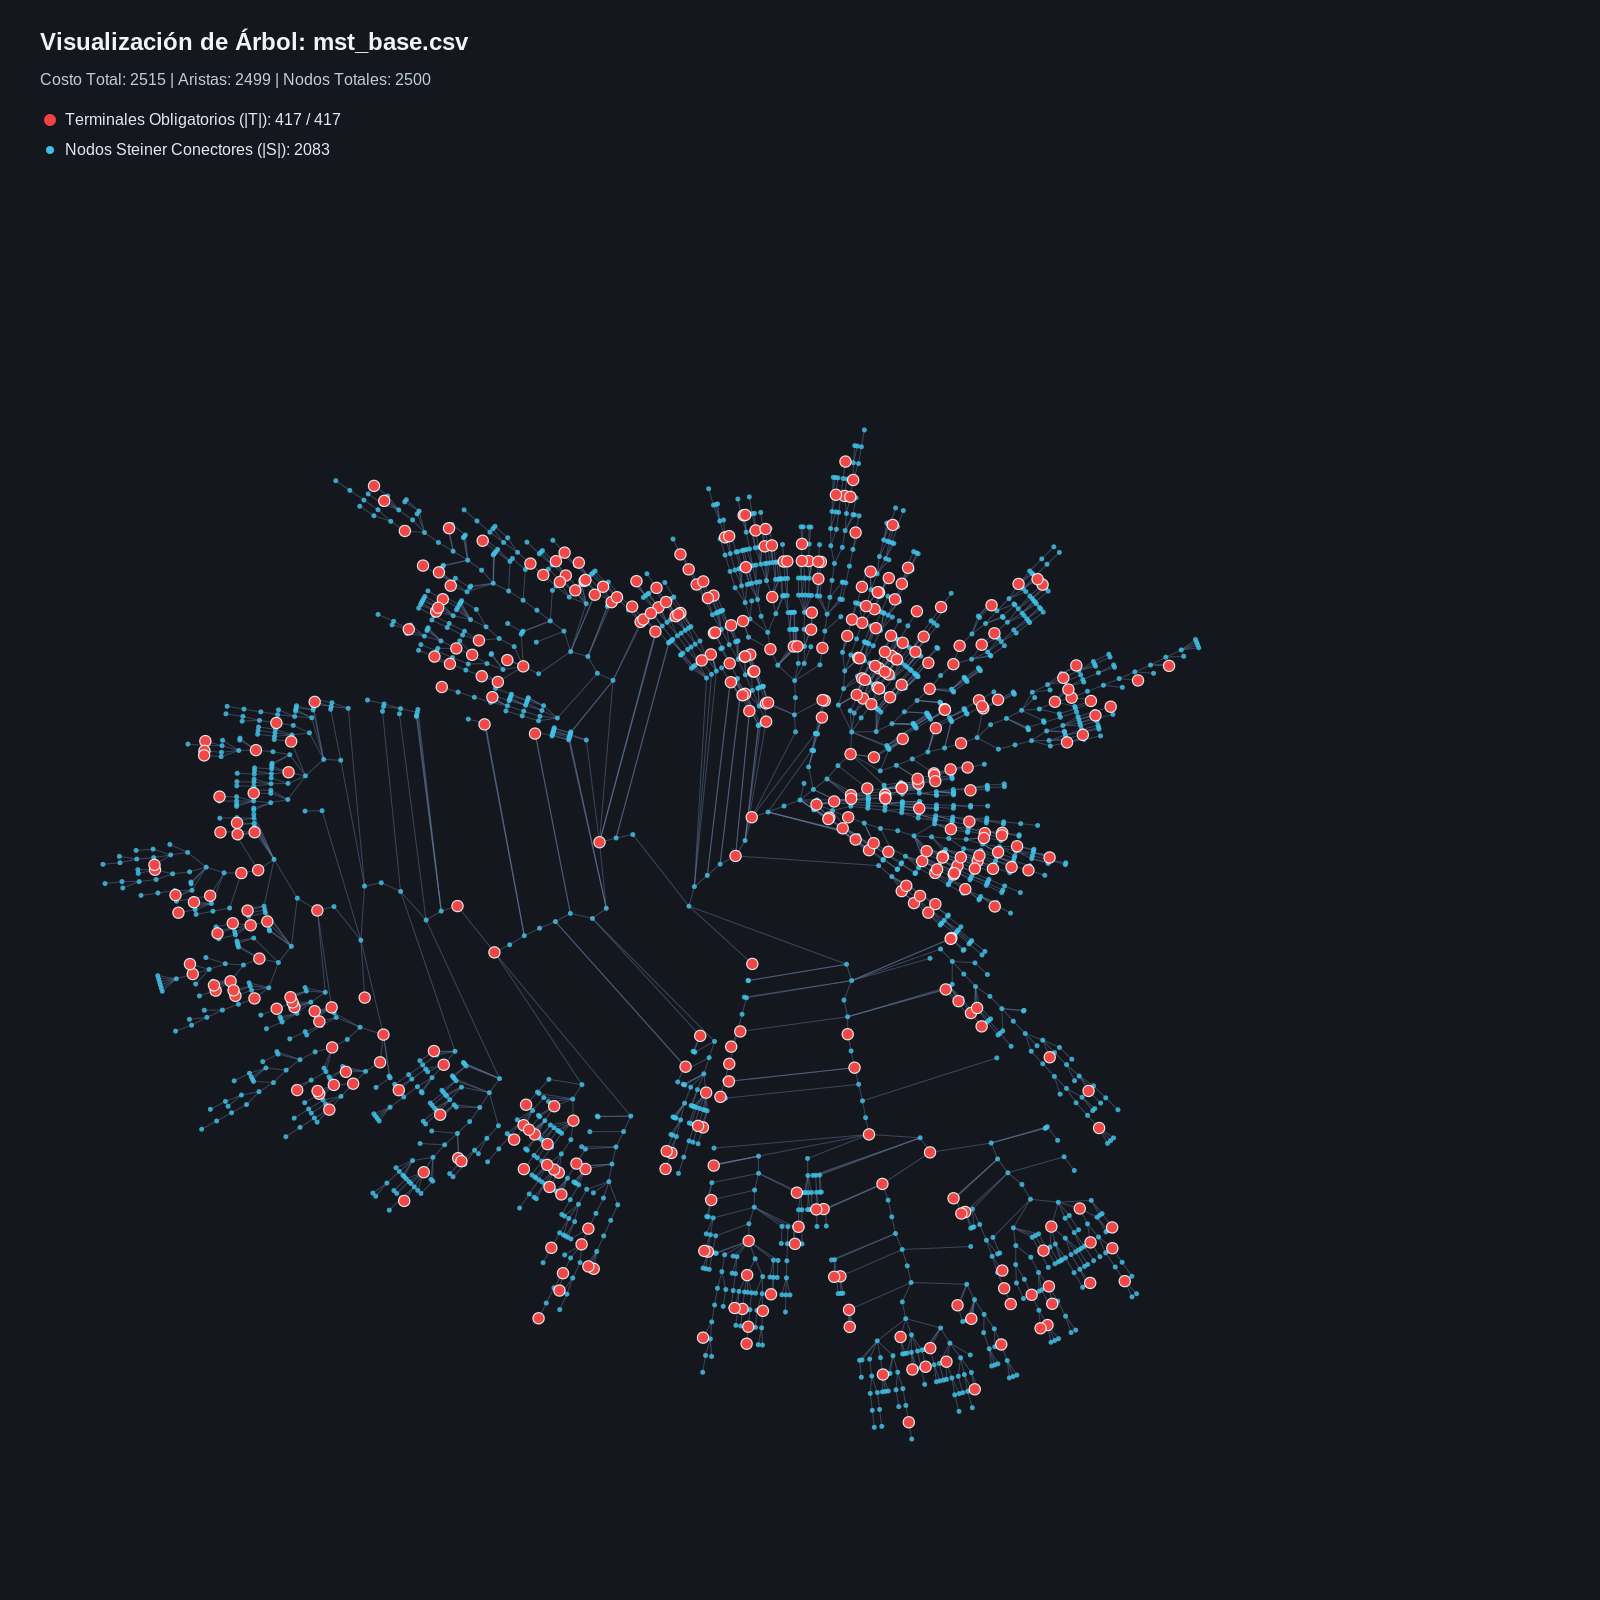
\includegraphics[width=\textwidth]{figures/mst_base.png}
        \caption{MST Base ($|E| = 2.499$, Costo $= 2.515$).}
        \label{fig:mst_base}
    \end{subfigure}
    \hfill
    \begin{subfigure}[b]{0.32\textwidth}
        \centering
        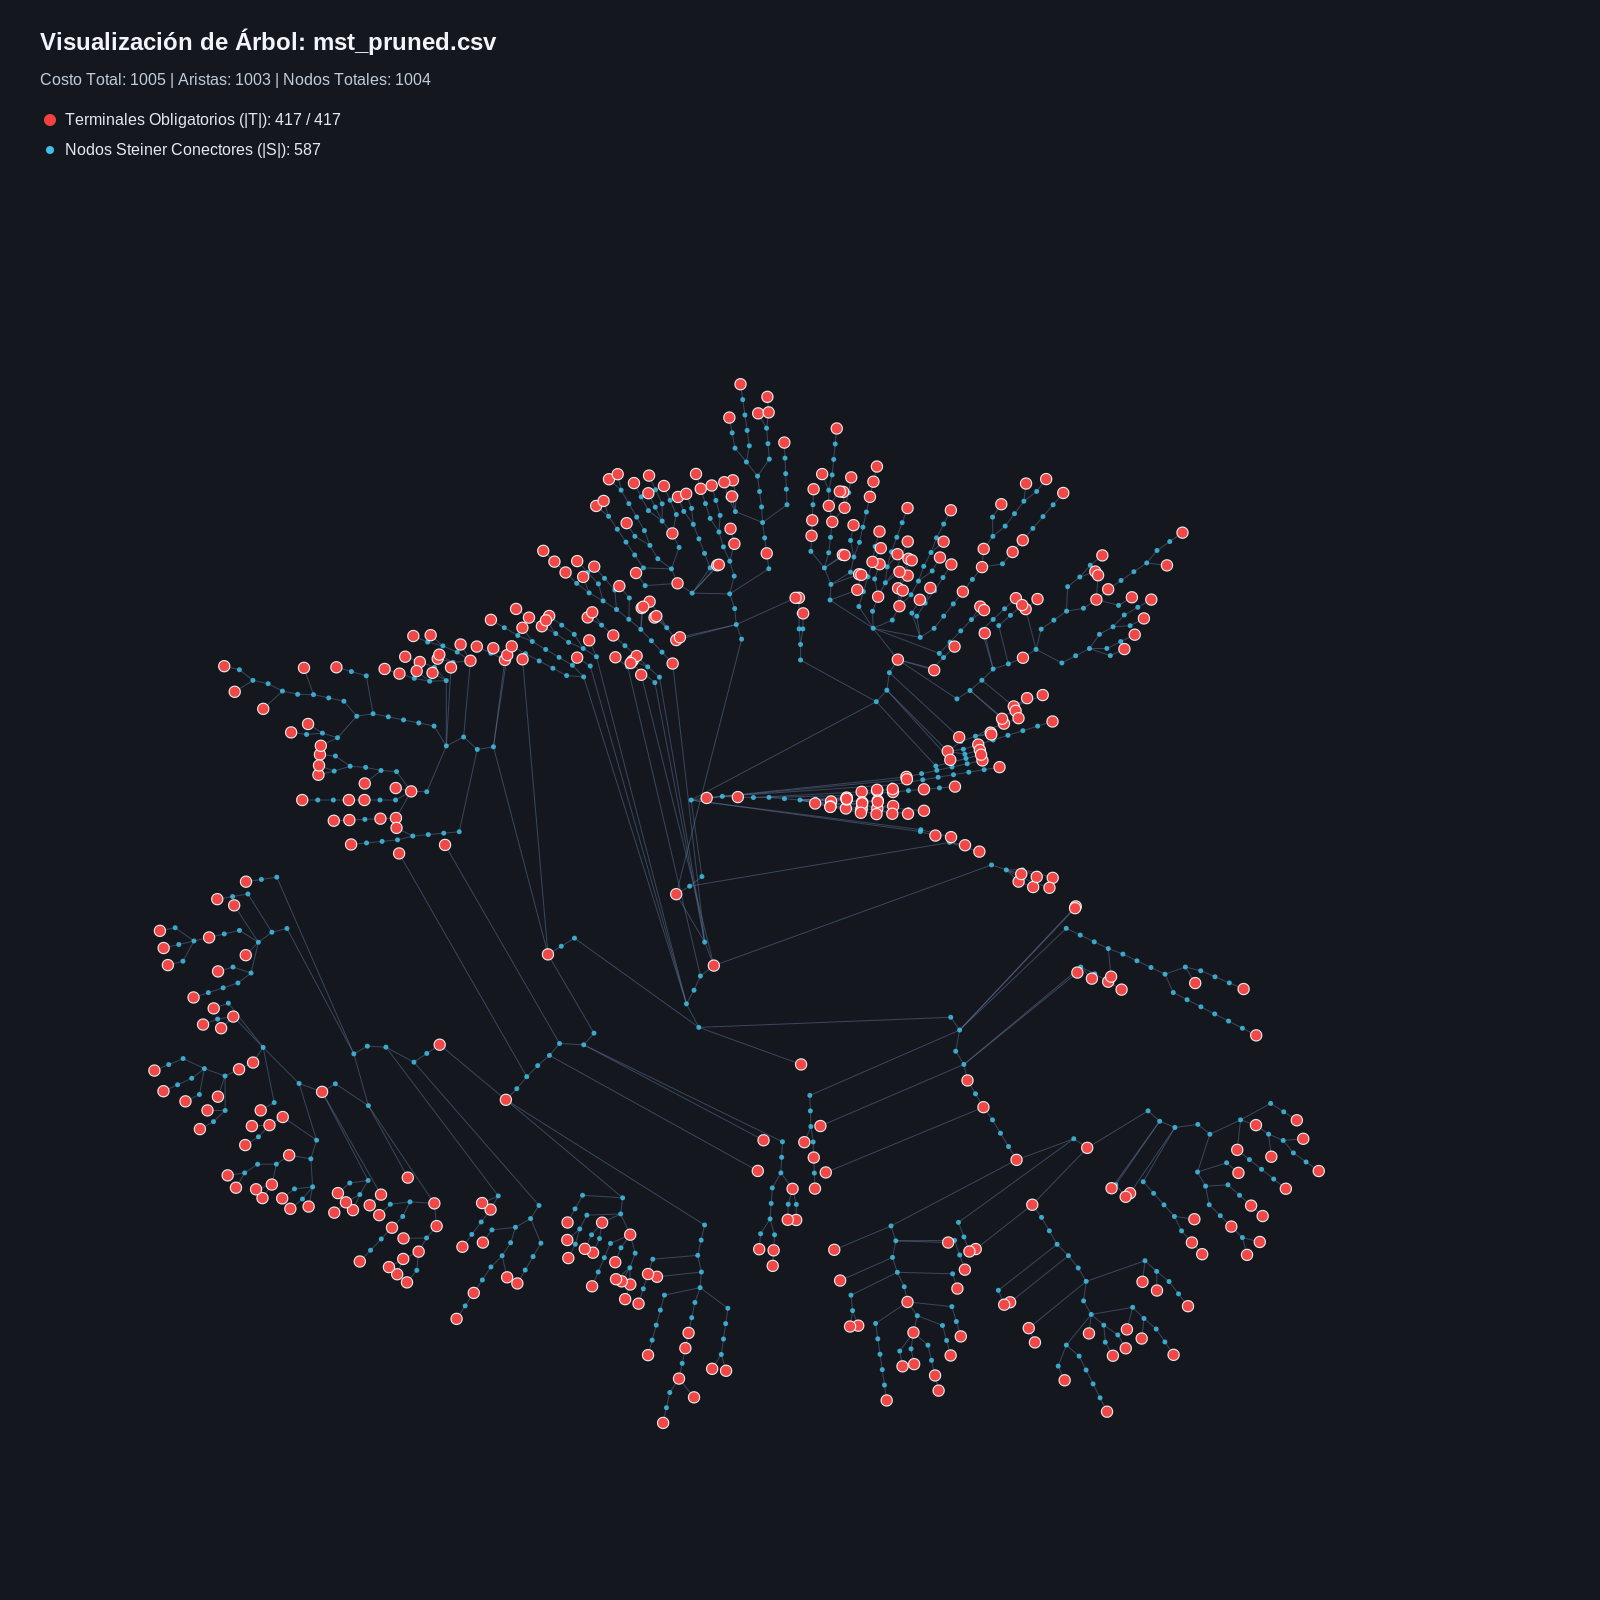
\includegraphics[width=\textwidth]{figures/mst_pruned.png}
        \caption{Kruskal Podado ($|E| = 1.003$, Costo $= 1.005$).}
        \label{fig:mst_pruned}
    \end{subfigure}
    \hfill
    \begin{subfigure}[b]{0.32\textwidth}
        \centering
        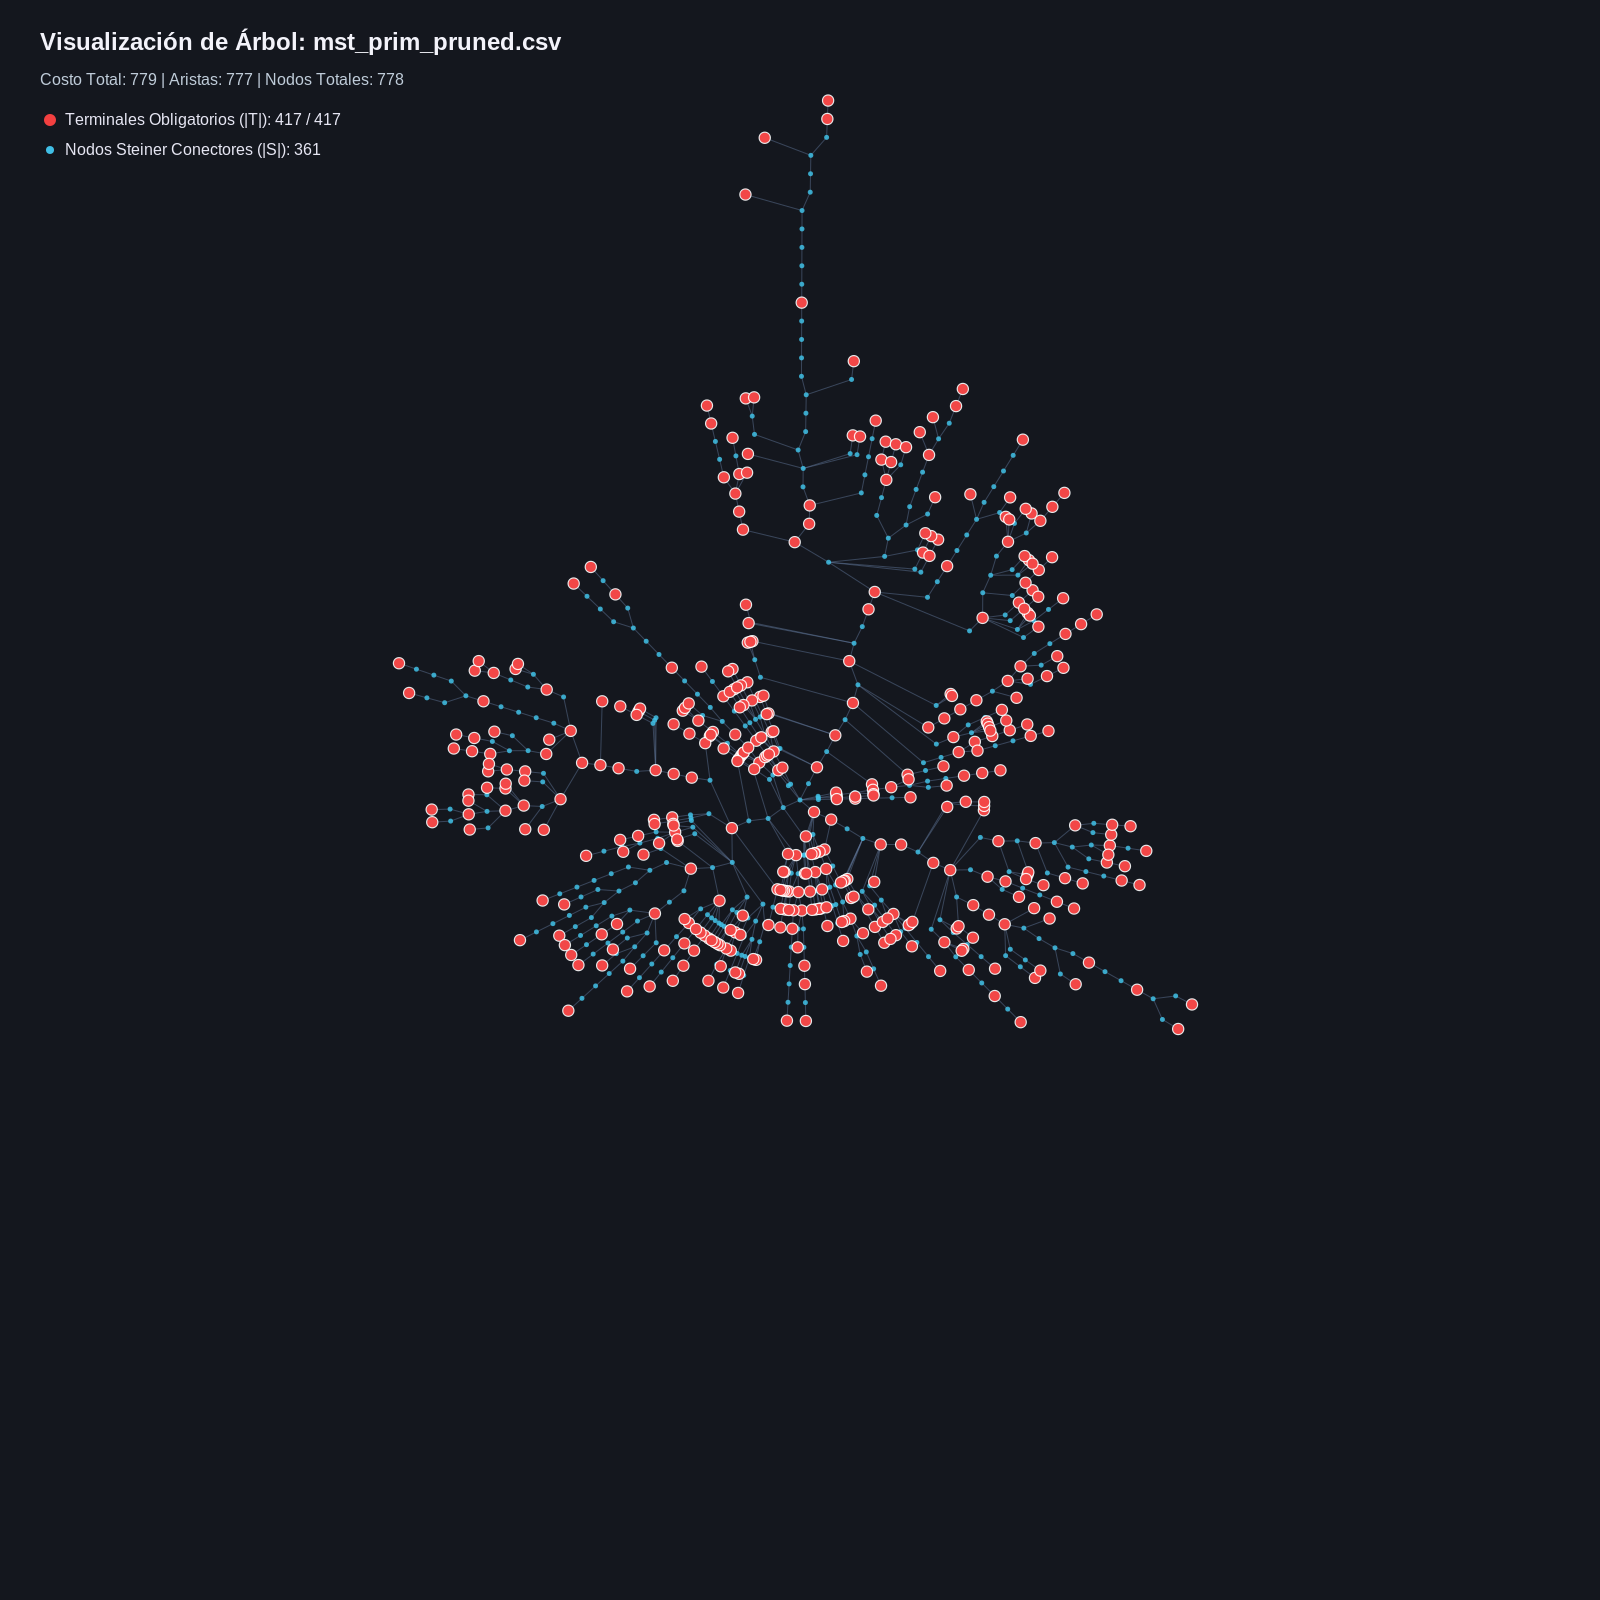
\includegraphics[width=\textwidth]{figures/mst_prim_pruned.png}
        \caption{Prim Podado ($|E| = 777$, Costo $= 779$).}
        \label{fig:mst_prim_pruned}
    \end{subfigure}
    \caption{Visualización gráfica de la reducción topológica: en rojo los $417$ terminales obligatorios y en celeste los nodos Steiner intermedios. Se constata la mayor compacidad de Prim orientado a terminales al reducir la red a $777$ aristas y costo $779$.}
    \label{fig:comparativa_visual}
\end{figure}

% ==============================================================================
% SECCIÓN 5: MÉTODO(S) DE MEJORA UTILIZADO(S)
% ==============================================================================
\section{Método(s) de Mejora Utilizado(s)}
\label{sec:heuristica}

\textit{[Sección asignada a Nicolas Montecino / Heurísticas y Optimización]}

\subsection{Heurística Constructiva basada en Caminos Mínimos (KMB / Mehlhorn)}
En lugar de calcular el MST sobre el grafo global y luego podarlo, las aproximaciones clásicas de alta calidad (como el algoritmo KMB \cite{kou1981fast} o Mehlhorn \cite{mehlhorn1988faster}) operan construyendo un grafo métrico reducido sobre los terminales obligatorios:
\begin{enumerate}
    \item Se calculan las distancias mínimas entre pares de terminales utilizando Dijkstra multi-fuente.
    \item Se construye el grafo completo métrico $G_M = (T, E_M)$.
    \item Se calcula el MST sobre $G_M$.
    \item Se reemplaza cada arista métrica por el camino mínimo original en $G$.
    \item Se extrae el MST del subgrafo resultante y se aplican las podas de hojas.
\end{enumerate}

\subsection{Búsqueda Local e Intercambio de Aristas}
\textit{[Detallar la estrategia de vecindad: reconexión de caminos, intercambio de nodos Steiner candidatos y criterios de parada o enfriamiento simulado para alcanzar el rango $\le 580$].}

% ==============================================================================
% SECCIÓN 6: RESULTADOS OBTENIDOS Y TIEMPOS
% ==============================================================================
\section{Resultados Obtenidos}
\label{sec:resultados}

\textit{[Sección asignada a Nicolas Montecino / Registro de Pruebas Experimentales]}

\subsection{Comportamiento Experimental}
\textit{[Presentar curvas de convergencia, número de iteraciones, uso de memoria y evolución del costo a lo largo de las ejecuciones del optimizador].}

% ==============================================================================
% SECCIÓN 7: COMPARACIÓN ENTRE SOLUCIONES
% ==============================================================================
\section{Comparación entre Soluciones}
\label{sec:comparacion}

\subsection{Consolidado Global de Métricas}
En la Tabla \ref{tab:resumen_global} se contrastan todos los métodos desarrollados contra los hitos de la rúbrica oficial de evaluación.

\begin{table}[htbp]
\centering
\small
\caption{Tabla comparativa global de resultados y ponderación según pauta oficial.}
\label{tab:resumen_global}
\begin{tabularx}{\textwidth}{lcccccX}
\toprule
\textbf{Método} & \textbf{Costo} & \textbf{Reducción \%} & \textbf{Gap vs Óptimo} & \textbf{Aristas} & \textbf{Tiempo} & \textbf{Pauta Oficial} \\
\midrule
MST Base (Kruskal / Prim) & $2.515$ & $0,00\%$ & $+345,9\%$ & $2.499$ & $\sim 4,8$ ms & 4 puntos \\
Kruskal Podado & $1.005$ & $-60,04\%$ & $+78,2\%$ & $1.003$ & $0,35$ ms & Factible (Poda inicial) \\
Prim Podado (Estándar) & $922$ & $-63,34\%$ & $+63,5\%$ & $920$ & $0,14$ ms & Factible \\
\textbf{Prim Podado (Desempate)} & $\mathbf{779}$ & $\mathbf{-69,03\%}$ & $\mathbf{+38,1\%}$ & $\mathbf{777}$ & $\mathbf{0,14\text{ ms}}$ & \textbf{Supera Hito 892 (5 pts)} \\
\textit{Hito Pauta (Poda Estructural)} & \textit{892} & \textit{-64,53\%} & \textit{+58,2\%} & \textit{-} & \textit{-} & \textit{5 puntos} \\
Heurística KMB & $[601, 891]$ & $-76,1\%$ a $-64,6\%$ & $+6,5\%$ a $+58\%$ & - & $< 1$ s & 6 - 7 puntos \\
Búsqueda Local & $[565, 580]$ & $-77,5\%$ a $-76,9\%$ & $\le +2,8\%$ & - & $< 10$ min & \textbf{11 - 14 puntos (Meta)} \\
\textbf{Óptimo SteinLib} & \textbf{564} & \textbf{-77,57\%} & \textbf{0,00\%} & \textbf{-} & \textbf{-} & \textbf{15 puntos (Máximo)} \\
\bottomrule
\end{tabularx}
\end{table}

\subsection{Análisis de Brecha (Gap)}
El Gap respecto al óptimo global conocido ($C^* = 564$) se calcula formalmente como:
\begin{equation}
    \text{Gap}(\%) = \frac{C_{\text{solución}} - C^*}{C^*} \times 100\%
\end{equation}

% ==============================================================================
% SECCIÓN 8: DIFICULTADES ENCONTRADAS
% ==============================================================================
\section{Dificultades Encontradas}
\label{sec:dificultades}

A lo largo del diseño, implementación y validación experimental del sistema, el equipo enfrentó los siguientes desafíos técnicos:
\begin{enumerate}
    \item \textbf{Estandarización de Formatos y Saltos de Línea:} La lectura del archivo \texttt{e18.stp} requirió una limpieza estricta de caracteres de retorno de carro (\texttt{\textbackslash r\textbackslash n}) para asegurar compatibilidad entre entornos Windows, Linux y WSL sin corromper el parser.
    \item \textbf{Indexación de Nodos en Base 1 vs. Base 0:} La convención oficial de SteinLib enumera los nodos desde $1$ hasta $2.500$. Se estructuraron los vectores internos con tamaño $N + 1$ para evitar desfases de índices entre módulos.
    \item \textbf{Verificación Formal de Aciclicidad:} Al reconectar caminos mínimos en la heurística, es común que se generen ciclos entre terminales adyacentes. Se requirió implementar un validador riguroso basado en DSU para certificar aciclicidad estricta ($|E| = |V| - 1$ y ausencia de lazos).
    \item \textbf{Escalabilidad de Algoritmos en Instancias Grandes:} Con $62.500$ aristas, el uso de matrices de adyacencia generaría una matriz densa inviable de $2.500 \times 2.500$ ($O(V^2)$). El uso de listas de adyacencia y colas de prioridad con Fibonacci o heap binario fue imperativo para sostener tiempos inferiores a $10$ ms.
\end{enumerate}

% ==============================================================================
% CONCLUSIONES
% ==============================================================================
\section{Conclusiones}
\label{sec:conclusiones}
La experimentación realizada demuestra la naturaleza contrastante entre los algoritmos de árbol generador mínimo y el problema del árbol de Steiner. Mientras que el MST se resuelve de forma determinista y en tiempo polinomial ($O(|E| \log |E|)$), el STPG exige discernir activamente cuáles nodos intermedios aportan beneficio marginal frente al costo de sus aristas incidentes. La poda iterativa de hojas constituye un mecanismo de alta eficiencia temporal que descarta más del $60\%$ del costo inicial sin comprometer la factibilidad.

% ==============================================================================
% BIBLIOGRAFÍA
% ==============================================================================
\bibliographystyle{plain}
\bibliography{references}

\end{document}
